\newcommand{\CLASSINPUTtoptextmargin}{1in}
\newcommand{\CLASSINPUTbottomtextmargin}{1in}
\newcommand{\CLASSINPUTinnersidemargin}{1in}
\newcommand{\CLASSINPUToutersidemargin}{1in}

\documentclass[10pt, conference, compsocconf]{IEEEtran}

\ifCLASSINFOpdf
  \usepackage[pdftex]{graphicx}
  \graphicspath{{./images/}}
  \DeclareGraphicsExtensions{.pdf,.jpeg,.png,.jpg}
\else
  \usepackage[dvips]{graphicx}
  \graphicspath{{./images/}}
  \DeclareGraphicsExtensions{.eps}
\fi

\begin{document}

\title{Usage Management of Personal Health Records}

\author{
\IEEEauthorblockN{Christopher C. Lamb, Rafael Figueroa, Rafael Fierro}
\IEEEauthorblockA{University of New Mexico\\
Department of Electrical and Computer Engineering\\
Albuquerque, NM 87131-0001 \\
\{cclamb, rafa, rfierro\}@ece.unm.edu}
}



\maketitle

\begin{abstract}
Insert abstract here.
\end{abstract}

%\begin{IEEEkeywords}
%usage management; personal health records
%\end{IEEEkeywords}
%\IEEEpeerreviewmaketitle

\section{Introduction}
Introduction to topic; why it is important, motivate reader.

\section{Cyber-physical Cloud Architectures}
Highlight the problem we are starting to address.

\subsection{A Taxonomoy of Architectures}
Outline an initial taxonomy.

\subsection{Initial Analysis of Taxonomy}
Notionally analyze the taxonomy.

\subsection{Future Work}
Where to next.

\section{Related Work}
Cover previous work in area, especially motivating work.

\section{Summary and Conclusions}

%\begin{figure}[!t]
%\centering
%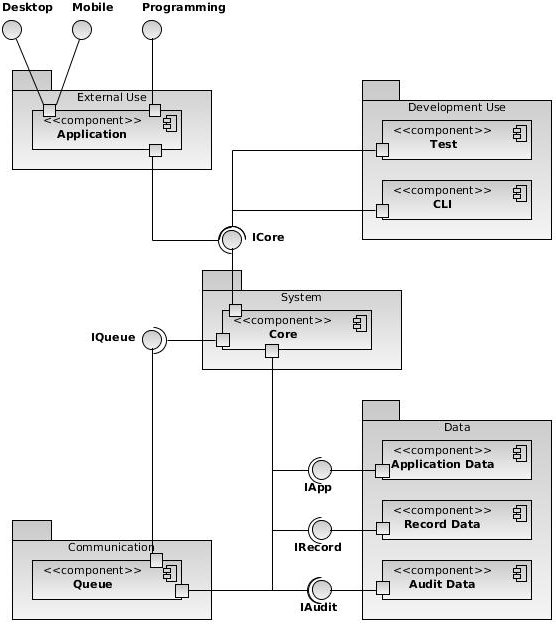
\includegraphics[width=3in]{HisbSystemArch}
%\caption{System Architecture Runtime Component View}
%\label{fig:RuntimeView}
%\end{figure}



\bibliographystyle{abbrv}
\bibliography{bib/cps.bib}

\end{document}


